\documentclass[a4,13pt]{extarticle}
\usepackage[utf8]{inputenc}
\usepackage[margin=2cm]{geometry}
\usepackage{amsmath}
\usepackage{graphicx}
\usepackage{algorithm}
\usepackage{algorithmicx}
\usepackage[]{algpseudocode}
\usepackage{hyperref}
\usepackage{color}

\definecolor{blue}{rgb}{0,0,0.5}
\newenvironment{Solution}{\color{blue}\textbf{Solution:}}{}

\title{COMP3506 Homework 1}
\author{Weighting: 15\%}
\date{Due date: 21st August 2020, 11:55 pm}

\begin{document}

\maketitle
\if 0
\section*{Overview}
This purpose of this assignment is for you to become familiar with understanding the main concepts and notation of asymptotic analysis of algorithms, to gain practice writing simple mathematical proofs, to learn how to read and write pseudocode algorithms, and to practice using binary search and writing and analysing recursive algorithms.

\section*{Marks}
This assignment is worth 15\% of your total grade. COMP3506 students will be marked on questions 1 to 4 out of \textbf{50 marks}. COMP7505 are required to additionally do question 5 and will be marked out of \textbf{60 marks}.\\\\
Partial marks \textit{may} be awarded for partially correct answers and answers lacking justification where it is required.

\section*{Submission Instructions}
\begin{itemize}
	\item Your answers to the written questions should be submitted as a file called \textbf{A1-[Your Student Number Here].pdf} via the \texttt{Homework 1 - Written} submission. Do not include your full name in your pdf submission.
	\item \textbf{Hand-written answers will not be marked.} If you are comfortable with the \LaTeX\  typesetting
	      system, it is strongly recommended that you write your answers using it, however it is not a requirement.
	\item Your solution to Q3a will be submitted via Gradescope to the \texttt{Homework 1 - Q3 Programming} submission. You should only submit your completed \texttt{ArrayCartesianPlane.java} file. No marks will be awarded for non-compiling submissions, or submissions which import non-supported 3rd party libraries. You should follow all constraints laid out in question 3 or risk losing marks for the question.
\end{itemize}

\section*{Late Submissions and Extensions}
Late submissions will not be accepted. It is your responsibility to ensure you have submitted your
work well in advance of the deadline (taking into account the possibility of computer, internet, or Gradescope
issues). You are allowed to submit multiple times, and only the latest submission before the deadline will be marked. See the ECP for information about extensions.
\section*{Academic Misconduct}
This assignment is an individual assignment. Posting questions or copying answers from the internet is considered cheating, as is sharing your answers with classmates. All your work (including code) will be analysed by sophisticated plagiarism detection software. \\\\
Students are reminded of the University’s policy on student misconduct, including plagiarism. See
the course profile and the School web page:
\url{http://www.itee.uq.edu.au/itee-student-misconduct-including-plagiarism}.\\

\newpage 

\fi 
\section*{Questions}

\begin{enumerate}
	\item   
	      Consider the following algorithm, \textsc{CoolAlgorithm}, which takes a \textbf{positive} integer $n$ and outputs another integer. 
	      Recall that `$\&$' indicates the bitwise AND operation and `$a >> b$' indicates the binary representation of $a$ shifted to the right $b$ times.
	      	      
	      \begin{algorithm}
	      	\begin{algorithmic}[1]
	      		\Procedure{CoolAlgorithm}{int n}
	      		\State $sum \gets 0$
	      		\If {$n$ \% $2 == 0$}
	      		\For{$i=0$ to $n$} 
	      		\For {$j=i$ to $n^2$}
	      		\State $sum \gets sum + i + j$ 
	      		\EndFor 
	      		\EndFor
	      		\Else
	      		\While{$n > 0$}
	      		\State $sum \gets sum$ + $(n$ \& $1)$
	      		\State $n \gets (n >> 1)$
	      		\EndWhile
	      		\EndIf
	      		\State \textbf{return} $sum$
	      		\EndProcedure
	      	\end{algorithmic}
	      \end{algorithm}
	      	          
	      Note that the runtime of the above algorithm depends not only on the size of the input $n$, but also on a numerical property of $n$. 
	      For all of the following questions, you must assume that $n$ is a positive integer.
	      	      
	      \begin{enumerate}
	      	\item (3 marks) Represent the running time (i.e. the number of primitive operations) of the algorithm 
	      	      when the input $n$ is \textbf{odd}, as a mathematical function called $T_{\text{odd}}(n)$. State all assumptions made and explain all your reasoning.
	      	      
	      	      \begin{Solution}
	      	      \end{Solution}
	      	      	      	                  
	      	\item (2 marks) Find a function $g(n)$ such that $T_{\text{odd}}(n)\in O(g(n))$. 
	      	      Your $g(n)$ should be such that the Big-O bound is as tight as possible (e.g. no constants or lower order terms). 
	      	      Using the formal definition of Big-O, prove this bound and explain all your reasoning. 
	      	      	      	                  
	      	      (Hint: you need to find values of $c$ and $n_0$ to prove the Big-O bound you gave is valid).
	      	      
	      	       \begin{Solution}
	      	      \end{Solution}
	      	      	      	                  
	      	\item (2 marks) Similarly, find the tightest Big-$\Omega$ bound of $T_{\text{odd}}(n)$ and use the formal definition of Big-$\Omega$ to prove the bound is correct. Does a Big-$\Theta$ bound for $T_{\text{odd}}(n)$ exist? If so, give it. If not, explain why it doesn't exist.
	      	
	      	\begin{Solution}
	      	\end{Solution}
	      	      	      	                  
	      	      	      	                  
	      	\item (3 marks) Represent the running time (as you did in part (a)) for the algorithm when the input $n$ is \textbf{even}, as a function called $T_{\text{even}}(n)$. State all assumptions made and explain all your reasoning. Also give a tight Big-O and Big-$\Omega$ bound on $T_{\text{even}}(n)$. You do \textbf{not} need to formally prove these bounds.
	      	
	      	\begin{Solution}
	      	\end{Solution}
	      	      	      	                  
	      	\item (2 marks) The running time for the algorithm has a best case and worst case, and which case occurs for a 
	      	      given input $n$ to the algorithm depends on the parity of $n$.
	      	      	      	                  
	      	      Give a Big-O bound on the \textbf{best case} running time of the algorithm, and a Big-$\Omega$ bound on 
	      	      the \textbf{worst case} running time of the algorithm (and state which parity of the input corresponds with which case).
	        \begin{Solution}
	      	\end{Solution}
	      	      	      	      
	      	      	      	                  
	      	\item (2 marks) We can represent the runtime of the entire algorithm, say $T(n)$, as
	      	      \begin{align*}
	      	      	T(n)=\begin{cases}
	      	      	T_{\text{even}}(n) & \text{if $n$ is even} \\
	      	      	T_{\text{odd}}(n)  & \text{if $n$ is odd}  \\
	      	      	\end{cases}
	      	      \end{align*}
	      	      Give a Big-$\Omega$ and Big-$O$ bound on $T(n)$ using your previous results. If a Big-$\Theta$ bound for the entire algorithm exists, describe it. If not, explain why it doesn’t exist.
	      	      
	      	\begin{Solution}
	      	\end{Solution}
	      	      	      	                  
	      	\item (2 marks) Your classmate tells you that Big-O represents the worst case runtime of an algorithm, and similarly that 
	      	      Big-$\Omega$ represents the best case runtime. Is your classmate correct? Explain why/why not. 
	      	      Your answers for (e) and (f) \textit{may} be useful for answering this.
	      	      
	      	\begin{Solution}
	      	\end{Solution}
	      	      	      	                  
	      	\item (1 mark) Prove that an algorithm runs in $\Theta (g(n))$ time if and only if its worst-case running time 
	      	      is $O(g(n))$ and its best-case running time is $\Omega(g(n))$.
	      	      
	      	\begin{Solution}
	      	\end{Solution}
	      	      	      	                  
	      \end{enumerate}
	      	          
	      \newpage 
	      	
	\item 
	      \begin{enumerate}
	      	\item (4 marks) Devise a \textbf{recursive} algorithm that takes a sorted array $A$ of length $n$, containing distinct (not necessarily positive) integers, and determines whether or not there is a position $i$ (where $0\leq i < n$) such that $A[i] = i$.
	      	      \begin{itemize}
	      	      	\item Write your algorithm in pseudocode (as a procedure called $\textsc{FindPosition}$ that takes an input array $A$ and returns a boolean).
	      	      	\item Your algorithm should be as efficient as possible (in terms of time complexity) for full marks.
	      	      	\item You will not receive any marks for an iterative solution for this question. 
	      	      	\item You are permitted (and even encouraged) to write helper functions in your solution.
	      	      \end{itemize}
	      	      
	      	\begin{Solution}
	      	\end{Solution}
	      	
	      	\item (1 mark) Show and explain all the steps taken by your algorithm (e.g. show all the recursive calls, if conditions, etc) for the following input array: $[-1,0,2,3,10,11,23,24,102]$.
	      	
	      	\begin{Solution}
	      	\end{Solution}
	      	      	      	                  
	      	\item (3 marks) Express the worst-case running time of your algorithm as a mathematical recurrence, $T(n)$, and explain your reasoning. 
	      	      Then calculate a Big-O (or Big-$\Theta$) bound for this recurrence and show all working used to find this bound 
	      	      (Note: using the Master Theorem below for this question will not give you any marks for this question).
	      	      
	      	      
	        \begin{Solution}
	      	\end{Solution}
	      	
	      	\item The master theorem is a powerful theorem that can be used to quickly calculate a tight asymptotic bound on a mathematical recurrence. A simplified version is stated as follows: Let $T(n)$ be a non-negative function that satisfies
	      	      \begin{align*}
	      	      	T(n)                              & = \begin{cases}    
	      	      	aT\left(\frac{n}{b}\right) + g(n) & \text{for $n > k$} \\
	      	      	c                                 & \text{for $n=k$}   
	      	      	\end{cases}
	      	      	\intertext{where $k$ is a non-negative integer, $a\geq 1$, $b\geq 2$, $c > 0$, and $g(n)\in \Theta(n^d)$ for $d\geq 0$. Then,}
	      	      	T(n)                              & \in \begin{cases}  
	      	      	\Theta(n^d)                       & \text{if $a<b^d$}  \\
	      	      	\Theta(n^d\log n)                 & \text{if $a=b^d$}  \\
	      	      	\Theta(n^{\log_b a})              & \text{if $a>b^d$}  
	      	      	\end{cases}
	      	      \end{align*}
	      	      \begin{enumerate}
	      	      	\item (1 mark) Use the master theorem, as stated above, to find a Big-$\Theta$ bound (and confirm your already found Big-O) for the recurrence you gave in (b). Show all your working.
	      	      	
	      	      	\begin{Solution}
	      	        \end{Solution}
	      	
	      	      	\item (1 mark) Use the master theorem to find a Big-$\Theta$ bound for the recurrence defined by $$T(n)=5 \cdot T\left(\frac{n}{3}\right) + n^2 + 2n$$ and $T(1)=100$. Show all working.
	      	      	      	
	      	      	\begin{Solution}
	      	        \end{Solution}
	      	
	      	      	\item (1 mark) Use the master theorem to find a Big-$\Theta$ bound for the recurrence defined by $$T(n)=8 \cdot T\left(\frac{n}{4}\right) + 5n + 2\log n +\frac 1n $$ and $T(1)=1$. Show all working.
	      	      	
	      	      	\begin{Solution}
	      	        \end{Solution}
	      	      \end{enumerate}
	      	      	      	                  
	      	\item (2 marks) Rewrite (in pseudocode) the algorithm you devised in part (a), but this time \textbf{iteratively}. 
	      	      Your algorithm should have the same runtime complexity of your recursive algorithm. Briefly explain how you determined the runtime complexity of your iterative solution.
	      	      
	      	\begin{Solution}
	      	\end{Solution}
	      	      	      	                  
	      	\item (2 marks) While both your algorithms have the same runtime complexity, one of them will usually be faster in practice 
	      	      (especially with large inputs) when implemented in a procedural programming language (such as Java, Python or C). 
	      	      Explain which version of the algorithm you would implement in Java - and why - if speed was the most important factor to you. 
	      	      You may need to do external research on how Java method calls work in order to answer this question in full detail. 
	      	      Cite any sources you used to come up with your answer.\\
	      	      	      	                  
	      	      In addition, explain and compare the space complexity of your both your recursive solution 
	      	      and your iterative solution (also assuming execution in a Java-like language).
	      	      
	        \begin{Solution}
	      	\end{Solution}
	      \end{enumerate}
	      	              
	      \newpage 
	      	          
	\item
	      In the support files for this homework on Blackboard, we have provided an interface called \texttt{CartesianPlane} which describes a 2D plane which can hold elements at $(x,y)$ coordinator pairs, where $x$ and $y$ could potentially be negative. 
	      \begin{enumerate}
	      	\item (5 marks) In the file \texttt{ArrayCartesianPlane.java}, you should implement the methods in the interface \texttt{CartesianPlane} using a multidimensional array as the underlying data structure.
	      	      	      	                      
	      	      Before starting, ensure you read and understand the following:
	      	      \begin{itemize}
	      	      		      	      	
	      	      	\item Your solution will be marked with an automated test suite. 
	      	      	      	      	      	                          
	      	      	\item Your code will be compiled using Java 11.
	      	      	      	      	      	                          
	      	      	\item Marks may be deducted for poor coding style. You should follow the CSSE2002 style guide, which can be found on Blackboard.
	      	      	      	      	      	                          
	      	      	\item  A sample test suite has been provided in \texttt{CartesianPlaneTest.java}. 
	      	      	      This test suite is not comprehensive and there is no guarantee that passing these will ensure passing 
	      	      	      the tests used during marking. It is recommended, but not required, that you write your own tests for your solution.
	      	      	      	      	    
	      	      	      	   	                          
	      	      	\item You may not use anything from the Java Collections Framework (e.g. ArrayLists or HashMaps). If unsure about whether you can use a certain import, ask on Piazza.
	      	      	                               
	      	      	\item Do not add or use any static member variables. Do not add any \textbf{public} variables or methods.
	      	      	\item Do not modify the interface (or \texttt{CartesianPlane.java} at all), or any method signatures in your implementation.
	      	      \end{itemize}
	      	      	      	                      
	      	\item (1 mark) State (using Big-O notation) the memory complexity of your implementation, 
	      	      ensuring you define all variables you use. Briefly explain how you came up with this bound.
	      	      
	        \begin{Solution}
	      	\end{Solution}
	      	      	      	                      
	      	\item (1 mark) Using the bound found above, evaluate the overall memory efficiency of your implementation. 
	      	      You should especially consider the case where your plane is very large but has very few elements.
	      	
	      	\begin{Solution}
	      	\end{Solution}
	      	      	      	                      
	      	\item (3 marks) State (using Big-O notation) the time complexity of the following methods:
	      	      	      	                      
	      	      \begin{itemize}
	      	      	\item \texttt{add}
	      	      	\item \texttt{get}
	      	      	\item \texttt{remove}
	      	      	\item \texttt{resize}
	      	      	\item \texttt{clear}
	      	      \end{itemize}
	      	      	      	                      
	      	      Ensure you define all variables used in your bounds, and briefly explain how you came up with the bounds. 
	      	      State any assumptions you made in determining your answers. You should simplify your bounds as much as possible.
	      	      
	      	\begin{Solution}
	      	\end{Solution}
	      \end{enumerate}
	      	              
	      	              
	      \newpage 
	      	
	\item  
	      The UQ water well company has marked out an $n\times n$ grid on a plot of land, in which their hydrologists know exactly 
	      one square has a suitable water source for a water well. They have access to a drill, which uses drill bits and can test one 
	      square at a time. Now, all they they need is a strategy to find this water source.
	      	         
	      Let the square containing the water source be $(s_x,s_y)$. After drilling in a square $(x,y)$, certain things can 
	      happen depending on where you drilled.
	      \begin{itemize}
	      	\item If $x > s_x$ or $y > s_y$, then the drill bit breaks and must be replaced.
	      	\item If $x=s_x$ or $y=s_y$, the hydrologists can determine which direction the water source is in.
	      \end{itemize}
	      	              
	      Note that both the above events can happen at the same time. Below is an example with $n=10$ and $(s_x, s_y)=(3, 4)$. 
	      The water source is marked with \textsf{\textbf{S}}. Drilling in a shaded square will break the drill bit, and drilling in 
	      a square with a triangle will reveal the direction.
	      \begin{center}
	      	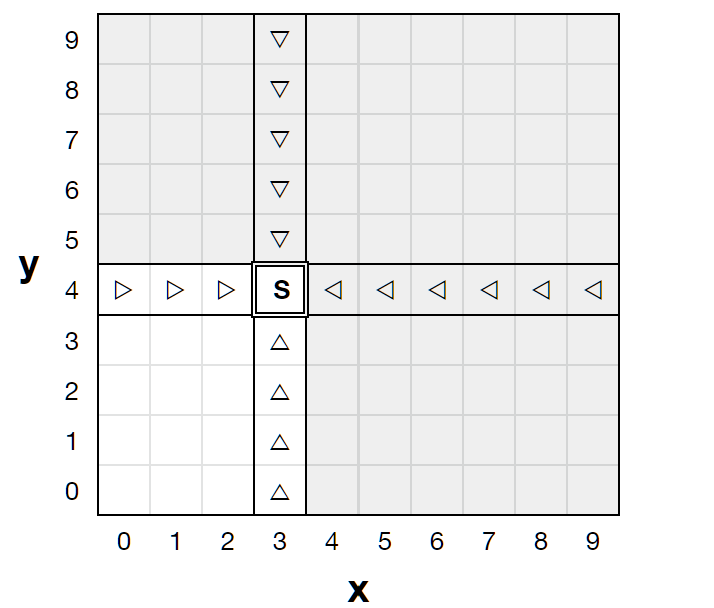
\includegraphics[width=0.4\textwidth]{a1q4new.png}
	      \end{center}
	      	              
	      \begin{enumerate} 
	      	\item (3 marks) The UQ water well company have decided to hire you - an algorithms expert - to devise a algorithm 
	      	      to find the water source as efficiently as possible. \\
	      	      	      	              
	      	      Describe (you may do this in words, but with sufficient detail) an algorithm to solve the problem of finding the water source, 
	      	      assuming you can break as many drill bits as you want. Provide a Big-O bound on the number of holes you need to drill to find 
	      	      it with your algorithm. Your algorithm should be as efficient as possible for full marks.\\\\
	      	      You may consult the hydrologists after any drill (and with a constant time complexity cost to do so) to see if 
	      	      the source is in the drilled row or column, and if so which direction the water source is in.\\\\
	      	      (Hint: A linear time algorithm is not efficient enough for full marks.)
	      	      
	      	\begin{Solution}
	      	\end{Solution}
	      	      	      	              
	      	\item 
	      	      (5 marks) The company, impressed with the drilling efficiency of your algorithm, assigns you to another $n \times n$ grid, 
	      	      which also has a water source you need to help find. However, due to budget cuts, this time you can only break $2$ drill 
	      	      bits (at most) before finding the source. (Note that you are able to use a $3$rd drill bit, but are not allowed to ever break it).
	      	      	      	              
	      	      Write \textbf{pseudocode} for an algorithm to find the source while breaking at most $2$ drill bits, and give a tight Big-O 
	      	      bound on the number of squares drilled (in the worst case). If you use external function calls (e.g. to consult the hydrologist, 
	      	      or to see if the cell you drilled is the source) you should define these, their parameters, and their return values. \\\\
	      	      Your algorithm's time complexity should be as efficient as possible in order to receive marks. 
	      	      (Hint: A linear time algorithm is not efficient enough for full marks.)
	      	      
	      	\begin{Solution}
	      	\end{Solution}
	      	      	      	              
	      \end{enumerate}
	      	              
	      	              
	      \newpage 
	\item 
	      \textbf{(COMP7505 only)} Binary search is fast because each step halves the search array. Can we do better? 
	      Maybe we could \textit{quarter} the input at every step. Would this make the algorithm faster?
	      	      
	      This ``quaternary search" algorithm takes a sorted array $A$ of length $n$ and an integer $x$. 
	      It determines which quarter of $A$ the value $x$ would occur in, then recurses into that subarray of length $n/4$. 
	      When reaching an array of length $n\le 4$, it returns the index of $x$ or $-1$ if $x$ cannot be found.
	      	              
	      \begin{enumerate}
	      	\item (3 marks) From the description above, write pseudocode for a quaternary search algorithm.
	      	
	      	\begin{Solution}
	      	\end{Solution}
	      	
	      	\item (1 mark) Express the worst case running time of quaternary search as a recurrence.
	      	
	      	
	      	\begin{Solution}
	      	\end{Solution}
	      	
	      	
	      	\item (2 marks) Solve the recurrence above to determine a Big-$O$ bound on the worst case running time of quaternary search.
	      	
	      	\begin{Solution}
	      	\end{Solution}
	      	
	      	\item (1 mark) Is quaternary search faster than binary search? If so, is it substantially faster? Explain briefly.
	      	
	      	\begin{Solution}
	      	\end{Solution}
	      	      	      	                  
	      	\item (3 marks) What if we go \textit{even further}? Suppose we can do $k$-ary search, which reduces $n$ to $n/k$ at each step (e.g.\ binary is $2$-ary search). With (c) in mind, we hypothesise that $k$-ary search has complexity $O(\log_k n)$.
	      	      	      	                  
	      	      Now, we can use $n$-ary search to search inside an $n$-length array. Our search finishes in one iteration because $n/n=1$ and $O(\log_n n) = O(1)$. We've solved algorithms! 
	      	      	      	                  
	      	      Unfortunately, nothing is that easy (or we wouldn't be here). Explain why this is \textit{not} the case and comment on the actual performance of $k$-ary search.
	      	      
	      	\begin{Solution}
	      	\end{Solution}
	      	      	      	                  
	      \end{enumerate}
	      	          
\end{enumerate}


\end{document}